\section{Changing Languages}

Sometimes, English just isn't the language you want. You might not speak English at all (in which case this guide isn't going to be much help), you might be more comfortable with another language or you might just be keen for a change. Whatever the reason, murcs (probably) has you covered, we took the time to add language support for every language we could find (and even a few that we couldn't).

To change the language, simply select the "View" menu (circled in red, below, for those stuck with a language they don't speak. It's always the third menu).

\begin{figure}[H]
\centering
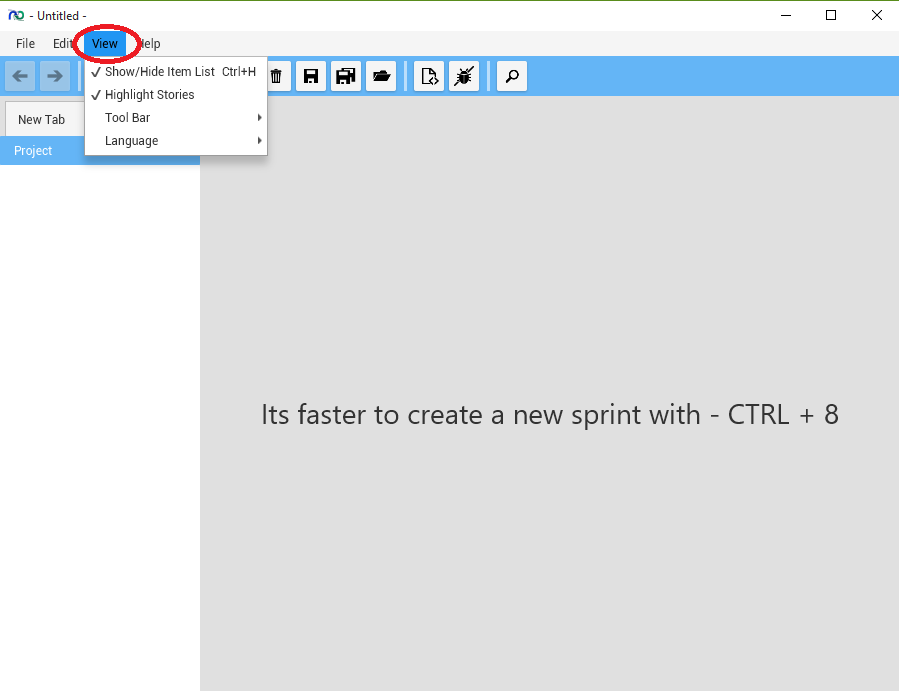
\includegraphics[width=\textwidth]{images/screenshots/language1.png}
\caption{The View Menu}
\label{fig:new_project}
\end{figure}

And select the "Language" submenu (circled below), which is at the bottom of the dropdown.

\begin{figure}[H]
\centering
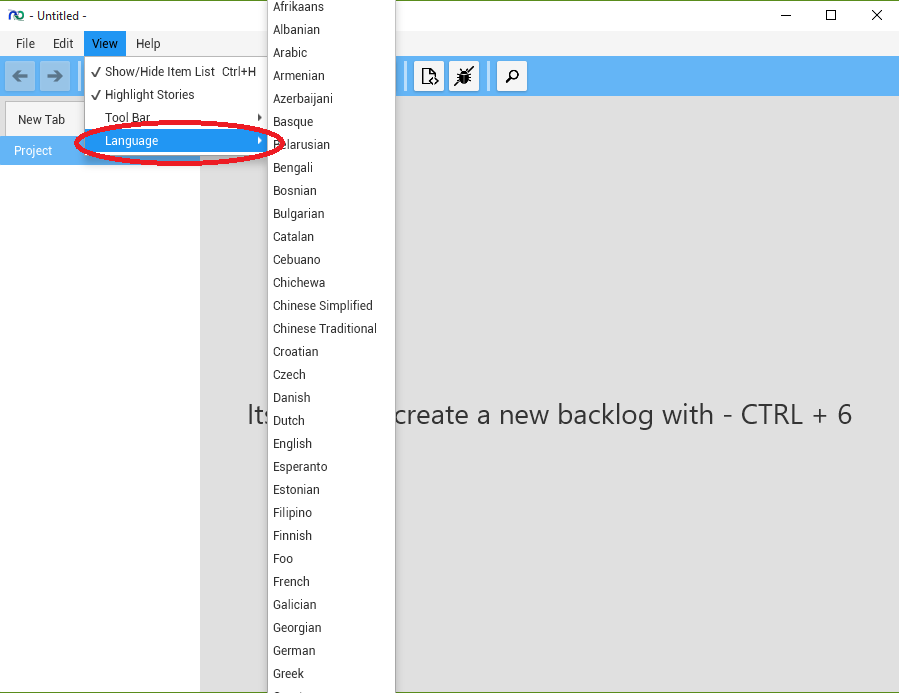
\includegraphics[width=\textwidth]{images/screenshots/language2.png}
\caption{The Language Menu}
\label{fig:new_project}
\end{figure}\textbf{}

Finally, pick the language that you want the application to change to. The application will change to it. You should note that any extra windows or tabs you have open will be closed, so you should make sure you have saved anything you're working on.